\documentclass[jou]{apa6}

\usepackage[american]{babel}

\usepackage{csquotes}
\usepackage[style=apa,sortcites=true,sorting=nyt,backend=biber]{biblatex}
\DeclareLanguageMapping{american}{american-apa}
\addbibresource{bibliography.bib}


%%%%%%%%%%%%%%%%%%%%%%%%%%%%%%%%%%%%%%%%
%% Discrete Structures
%% The start of RBS stuff
%%%%%%%%%%%%%%%%%%%%%%%%%%%%%%%%%%%%%%%%

% Working internal and external links in PDF
\usepackage{hyperref}
% Extra math symbols in LaTeX
\usepackage{amsmath}
\usepackage{gensymb}
\usepackage{amssymb}
% Enumerations with (a), (b), etc.
\usepackage{enumerate}
\usepackage[framemethod=TikZ]{mdframed}
\usepackage{xcolor}
\usepackage{graphicx}
\usepackage[justification=centering]{caption}
\usepackage{fancyvrb}
%\usepackage{changepage}
\usepackage{caption}% http://ctan.org/pkg/caption
\captionsetup[table]{format=plain,labelformat=simple,labelsep=period}%

\def\changemargin#1#2{\list{}{\rightmargin#2\leftmargin#1}\item[]}
\let\endchangemargin=\endlist 


\let\OLDitemize\itemize
\renewcommand\itemize{\OLDitemize\addtolength{\itemsep}{-6pt}}

\usepackage{etoolbox}
\makeatletter
\preto{\@verbatim}{\topsep=3pt \partopsep=3pt }
\makeatother

% These sizes redefine APA for A4 paper size
\oddsidemargin 0.0in
\evensidemargin 0.0in
\textwidth 6.27in
\headheight 1.0in
%\topmargin -24pt
\topmargin -32pt
\headheight 12pt
\headsep 12pt
%\textheight 9.19in
\textheight 9.35in


\title{Sample Quiz 8}
\author{Discrete Structures, Spring 2020}
\affiliation{RBS}

\leftheader{Discrete Sample Quiz 8}

\abstract{%
}

%\keywords{}

\setlength\parindent{0pt}

\begin{document}

\twocolumn
\thispagestyle{empty}

\begin{center}
{\Large Alternative Homework 1:}\\
{\Large Information Compression}
\end{center}

% https://ocw.mit.edu/courses/electrical-engineering-and-computer-science/6-441-information-theory-spring-2016/assignments/

\begin{changemargin}{10pt}{10pt}
{\footnotesize
{\em Note.} This is derived from MIT OCW content.\\
See \url{https://ocw.mit.edu/terms/}. 
The original assignments and related materials can be retrieved from two MIT courses:
\url{https://bit.ly/37Aywtf} and \url{https://bit.ly/2BdK8GA}\\
}
\end{changemargin}


{\bf Question 1.} 
Run-length encoding is a popular variable-length lossless compressor used in fax machines, image
compression, etc. 
In this problem consider compression of $X^n$ \textendash{} an i.i.d. (independent, identically distributed) sequences 
of $n$ bits. 
Here one message $X$ is a Bernoulli random variable with very small probability to get value $1$ 
(namely, $P(X=1) = \frac{1}{100}$ and the probability to get value $0$ is $P(X=0) = \frac{99}{100}$). 


We encode sequences of $n$ such messages $X^n$ using run-length encoding function $f(X^n)$ that is defined on $X^n$ 
(any sequence of $n$ bits) and follows these rules:
\begin{enumerate}
\item A chunk of consecutive $r \leq 128$ zeros (resp.\ ones) 
is encoded as one bit equal to $\mathtt{0}$ (resp.\ $\mathtt{1}$) followed by an $7$-bit binary encoding of $r$. 
(Therefore, the length of the encoding of a single chunk is exactly $8$ bits.)
\item If the input contains 
a run $r>128$ (more than $128$ consecutive zeros or ones), then split this into multiple chunks where the last chunk 
can be shorter than $128$ bits. Encode every chunk as described in the previous step.
\end{enumerate}
Compute the average achieved compression rate
$$\lim_{n \rightarrow \infty} \frac{1}{n} E(\ell(f(X^n)).$$

This formula shows the expected value $E$ of the random variable $\ell(f(X^n))$, where 
$\ell$ denotes the length of the encoded (compressed) message. 
How does it compare with the optimal lossless compressor? 
Compute both code lengths in bits (and round them up to the precision $10^{-5}$).

(This is a parody of Exercise 4, see \url{https://bit.ly/2Y6mUKa}.)



\vspace{10pt}
{\bf Question 2.} 
A source with an alphabet size of $M = |X| = 4$ has symbol probabilities $\{1/3, 1/3, 2/9, 1/9\}$.
 
\begin{enumerate}
\item Use the Huffman algorithm to find an optimal prefix-free code for this source.
\item Use the Huffman algorithm to find another optimal prefix-free code with a different set
of lengths.
\item Find another prefix-free code that is optimal but cannot result from using the Huffman
algorithm. 
\end{enumerate}

This is an exact copy of 2.12. See \url{https://bit.ly/2Y4PKMe}, page 55.


\vspace{10pt}
{\bf Question 3.}\\
Assume that the Markov process (Figure~\ref{fig:markov-chain}) has already reached a steady state,
(this means that we have done a sufficiently long random walk in this probabilistic graph and the 
starting state does not affect the probability distributions).

\begin{figure}[!htb]
\center{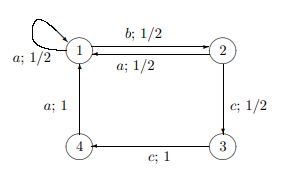
\includegraphics[width=2.6in]{alt-hw01/markov-chain.png}}
\caption{\label{fig:markov-chain} Markov chain.}
\end{figure}


The corresponding Markov source $X$ generates messages from the alphabet $\{a, b, c\}$
with certain probabilities. Sequences of messages from $X^n$ (sequences of $n$ letters where you 
can assume than $n$ is an even number) are compressed 
by two different people in two different ways:
\begin{enumerate}
\item Alice uses Arithmetic encoding to compress individual messages from the alphabet $\{a, b, c\}$. 
Find the average number of bits that Alice spends per {\bf one} message.
\item Bob first splits the sequence $X^n$ into pairs and then 
uses Arithmetic encoding to compress pairs of messages $\{aa, ab, ac, ba, bb, bc, ca,cb,cc\}$
(some pairs may be impossible). 
Find the average number of bits that Bob spends per {\bf one} message.
\end{enumerate}




This is a parody of problem 2.30. See \url{https://bit.ly/2Y4PKMe}, page 60.
(Arithmetic coding and its code length is defined in the textbook by G.Blelloch, see \url{https://bit.ly/2N3ywsf}.) 

% https://ocw.mit.edu/courses/electrical-engineering-and-computer-science/6-450-principles-of-digital-communications-i-fall-2006/index.htm


%https://ocw.mit.edu/courses/electrical-engineering-and-computer-science/6-441-information-theory-spring-2016/assignments/MIT6_441S16_problem_set3.pdf



% https://ocw.mit.edu/courses/electrical-engineering-and-computer-science/6-050j-information-and-entropy-spring-2008/
%% Entropy related theory.

% https://ocw.mit.edu/courses/electrical-engineering-and-computer-science/6-441-information-theory-spring-2016/lecture-notes/
%% Lossy compression


% https://ocw.mit.edu/courses/electrical-engineering-and-computer-science/6-004-computation-structures-spring-2017/c1/
%% Some very easy exercises on coding.


% https://ocw.mit.edu/courses/electrical-engineering-and-computer-science/6-02-introduction-to-eecs-ii-digital-communication-systems-fall-2012/lecture-slides/
%% LZW encoding and similar










\end{document}

